% Options for packages loaded elsewhere
% Options for packages loaded elsewhere
\PassOptionsToPackage{unicode}{hyperref}
\PassOptionsToPackage{hyphens}{url}
%
\documentclass[
  10pt,
  ignorenonframetext,
  aspectratio=169,
  russian,
]{beamer}
\newif\ifbibliography
\usepackage{pgfpages}
\setbeamertemplate{caption}[numbered]
\setbeamertemplate{caption label separator}{: }
\setbeamercolor{caption name}{fg=normal text.fg}
\beamertemplatenavigationsymbolshorizontal
% remove section numbering
\setbeamertemplate{part page}{
  \centering
  \begin{beamercolorbox}[sep=16pt,center]{part title}
    \usebeamerfont{part title}\insertpart\par
  \end{beamercolorbox}
}
\setbeamertemplate{section page}{
  \centering
  \begin{beamercolorbox}[sep=12pt,center]{section title}
    \usebeamerfont{section title}\insertsection\par
  \end{beamercolorbox}
}
\setbeamertemplate{subsection page}{
  \centering
  \begin{beamercolorbox}[sep=8pt,center]{subsection title}
    \usebeamerfont{subsection title}\insertsubsection\par
  \end{beamercolorbox}
}
% Prevent slide breaks in the middle of a paragraph
\widowpenalties 1 10000
\raggedbottom
\AtBeginPart{
  \frame{\partpage}
}
\AtBeginSection{
  \ifbibliography
  \else
    \frame{\sectionpage}
  \fi
}
\AtBeginSubsection{
  \frame{\subsectionpage}
}
\usepackage{iftex}
\ifPDFTeX
  \usepackage[T1]{fontenc}
  \usepackage[utf8]{inputenc}
  \usepackage{textcomp} % provide euro and other symbols
\else % if luatex or xetex
  \usepackage{unicode-math} % this also loads fontspec
  \defaultfontfeatures{Scale=MatchLowercase}
  \defaultfontfeatures[\rmfamily]{Ligatures=TeX,Scale=1}
\fi
\usepackage{lmodern}

\usetheme[]{metropolis}
\usefonttheme{serif} % use mainfont rather than sansfont for slide text
\ifPDFTeX\else
  % xetex/luatex font selection
  \setmainfont[]{DejaVu Sans}
  \setsansfont[]{DejaVu Sans}
  \setmonofont[]{DejaVu Sans Mono}
\fi
% Use upquote if available, for straight quotes in verbatim environments
\IfFileExists{upquote.sty}{\usepackage{upquote}}{}
\IfFileExists{microtype.sty}{% use microtype if available
  \usepackage[]{microtype}
  \UseMicrotypeSet[protrusion]{basicmath} % disable protrusion for tt fonts
}{}


\usepackage{longtable,booktabs,array}
\newcounter{none} % for unnumbered tables
\usepackage{calc} % for calculating minipage widths
\usepackage{caption}
% Make caption package work with longtable
\makeatletter
\def\fnum@table{\tablename~\thetable}
\makeatother
\usepackage{graphicx}
\makeatletter
\newsavebox\pandoc@box
\newcommand*\pandocbounded[1]{% scales image to fit in text height/width
  \sbox\pandoc@box{#1}%
  \Gscale@div\@tempa{\textheight}{\dimexpr\ht\pandoc@box+\dp\pandoc@box\relax}%
  \Gscale@div\@tempb{\linewidth}{\wd\pandoc@box}%
  \ifdim\@tempb\p@<\@tempa\p@\let\@tempa\@tempb\fi% select the smaller of both
  \ifdim\@tempa\p@<\p@\scalebox{\@tempa}{\usebox\pandoc@box}%
  \else\usebox{\pandoc@box}%
  \fi%
}
% Set default figure placement to htbp
\def\fps@figure{htbp}
\makeatother



\ifLuaTeX
\usepackage[bidi=basic,shorthands=off,provide=*]{babel}
\else
\usepackage[bidi=default,shorthands=off,provide=*]{babel}
\fi
\ifPDFTeX
\else
\babelfont{rm}[]{DejaVu Sans}
\fi
\ifLuaTeX
  \usepackage{selnolig} % disable illegal ligatures
\fi


\setlength{\emergencystretch}{3em} % prevent overfull lines

\providecommand{\tightlist}{%
  \setlength{\itemsep}{0pt}\setlength{\parskip}{0pt}}



 

\usepackage[]{csquotes}

%%% Load theme
\IfFileExists{beamerthemegotham.sty}{
  %%%% Full TeXlive
  \usetheme{gotham}
  \gothamset{
    numbering=totalframenumber,
    parttocframe default=off,
    sectiontocframe default=off,
    subsectiontocframe default=off,
    tocframe template=gotham bullet,
    % progressbar position=frametitle,
    progressbar position=foot,
  }
  \renewcommand{\gothamInstituteLogoSquare}[1][4ex]{%
    
\includegraphics[height=##1]{_resources/image/logo_rudn-inverted.png}
  }
  % \renewcommand{\gothamtitlepagelogo}[1][4ex]{%
  %   
\includegraphics[height=##1]{_resources/image/logo_rudn.png}
  % }
}{%
  %%%% TinyTeX
  \usepackage{libertine}
  %%%% https://deic.uab.cat/~iblanes/beamer_gallery/
  \usetheme{Madrid}
}
\metroset{progressbar=frametitle,numbering=fraction}
\setbeamersize{text margin left=8mm,text margin right=8mm}
\makeatletter
\@ifpackageloaded{caption}{}{\usepackage{caption}}
\AtBeginDocument{%
\ifdefined\contentsname
  \renewcommand*\contentsname{Содержание}
\else
  \newcommand\contentsname{Содержание}
\fi
\ifdefined\listfigurename
  \renewcommand*\listfigurename{Список иллюстраций}
\else
  \newcommand\listfigurename{Список иллюстраций}
\fi
\ifdefined\listtablename
  \renewcommand*\listtablename{Список таблиц}
\else
  \newcommand\listtablename{Список таблиц}
\fi
\ifdefined\figurename
  \renewcommand*\figurename{Рисунок}
\else
  \newcommand\figurename{Рисунок}
\fi
\ifdefined\tablename
  \renewcommand*\tablename{Таблица}
\else
  \newcommand\tablename{Таблица}
\fi
}
\@ifpackageloaded{float}{}{\usepackage{float}}
\floatstyle{ruled}
\@ifundefined{c@chapter}{\newfloat{codelisting}{h}{lop}}{\newfloat{codelisting}{h}{lop}[chapter]}
\floatname{codelisting}{Список}
\newcommand*\listoflistings{\listof{codelisting}{Листинги}}
\makeatother
\makeatletter
\makeatother
\makeatletter
\@ifpackageloaded{caption}{}{\usepackage{caption}}
\@ifpackageloaded{subcaption}{}{\usepackage{subcaption}}
\makeatother

\usepackage{bookmark}
\IfFileExists{xurl.sty}{\usepackage{xurl}}{} % add URL line breaks if available
\urlstyle{same}
% fallback for those not using the hyperref driver hyperxmp:
\makeatletter
\@ifundefined{xmpquote}{\newcommand{\xmpquote}[1]{#1}}{}
\makeatother
\hypersetup{
  pdftitle={Лабораторная работа №8},
  pdfauthor={Нечаева Кира Андреевна},
  pdflang={ru-RU},
  hidelinks,
  pdfcreator={LaTeX via pandoc}}


\title{\texorpdfstring{Лабораторная работа №8}{Лабораторная работа №8}}
\subtitle{\texorpdfstring{Модель конкуренции двух
фирм}{Модель конкуренции двух фирм}}
\author{Нечаева Кира Андреевна}
\date{}
\institute{НКНбд-01-23}

\begin{document}
\frame{\titlepage}


\begin{frame}{Постановка задачи}
\protect\phantomsection\label{ux43fux43eux441ux442ux430ux43dux43eux432ux43aux430-ux437ux430ux434ux430ux447ux438}
\textbf{Вариант 2}

Начальные оборотные средства:

\[
M_1(0)=1.9,
\qquad
M_2(0)=2.1.
\]

Необходимо сравнить:

\begin{enumerate}
\tightlist
\item
  чисто рыночную конкуренцию;
\item
  конкуренцию с дополнительным социально-психологическим фактором.
\end{enumerate}
\end{frame}

\begin{frame}{Исходные параметры}
\protect\phantomsection\label{ux438ux441ux445ux43eux434ux43dux44bux435-ux43fux430ux440ux430ux43cux435ux442ux440ux44b}
\begin{columns}[T]
\begin{column}{0.5\linewidth}
\[
p_{cr}=25,
\qquad
N=50,
\qquad
q=1
\]

\[
\tau_1=30,
\qquad
\tau_2=20
\]
\end{column}

\begin{column}{0.5\linewidth}
\[
p_1=7,
\qquad
p_2=10
\]

\(M_1\), \(M_2\) --- оборотные средства фирм.

Используется безразмерное время

\[
\theta=\frac{t}{c_1}.
\]
\end{column}
\end{columns}
\end{frame}

\begin{frame}{Коэффициенты модели}
\protect\phantomsection\label{ux43aux43eux44dux444ux444ux438ux446ux438ux435ux43dux442ux44b-ux43cux43eux434ux435ux43bux438}
Коэффициенты рассчитываются программно из исходных параметров:

\[
a_1\approx1.13\cdot10^{-5},
\qquad
a_2=1.25\cdot10^{-5},
\]

\[
b\approx2.83\cdot10^{-10},
\]

\[
c_1\approx0.0857,
\qquad
c_2=0.075.
\]

Ручная подстановка коэффициентов не требуется.
\end{frame}

\begin{frame}{Случай 1: рыночная конкуренция}
\protect\phantomsection\label{ux441ux43bux443ux447ux430ux439-1-ux440ux44bux43dux43eux447ux43dux430ux44f-ux43aux43eux43dux43aux443ux440ux435ux43dux446ux438ux44f}
Для первой фирмы:

\[
\frac{dM_1}{d\theta}
=
M_1-\frac{b}{c_1}M_1M_2-\frac{a_1}{c_1}M_1^2.
\]

Для второй фирмы:

\[
\frac{dM_2}{d\theta}
=
\frac{c_2}{c_1}M_2
-\frac{b}{c_1}M_1M_2
-\frac{a_2}{c_1}M_2^2.
\]
\end{frame}

\begin{frame}{Результат первого случая}
\protect\phantomsection\label{ux440ux435ux437ux443ux43bux44cux442ux430ux442-ux43fux435ux440ux432ux43eux433ux43e-ux441ux43bux443ux447ux430ux44f}
\begin{columns}[c]
\begin{column}{0.35\linewidth}
К концу интервала:

\[
M_1\approx7559.85,
\]

\[
M_2\approx5999.83.
\]

Обе фирмы сохраняются на рынке.
\end{column}

\begin{column}{0.65\linewidth}
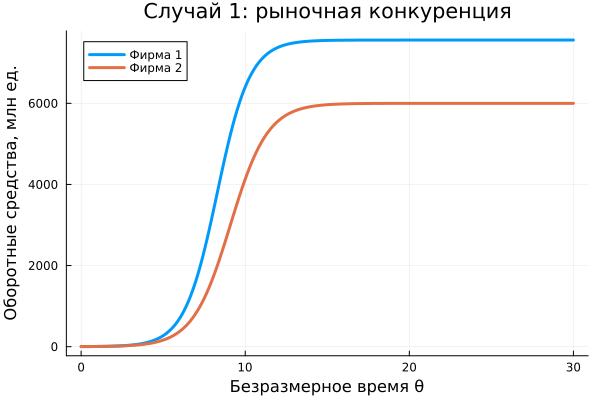
\includegraphics[width=1\linewidth,height=\textheight,keepaspectratio]{image/case1.png}
\end{column}
\end{columns}
\end{frame}

\begin{frame}{Случай 2: дополнительный фактор}
\protect\phantomsection\label{ux441ux43bux443ux447ux430ux439-2-ux434ux43eux43fux43eux43bux43dux438ux442ux435ux43bux44cux43dux44bux439-ux444ux430ux43aux442ux43eux440}
В первом уравнении коэффициент взаимодействия изменяется:

\[
\frac{b}{c_1}
\quad\longrightarrow\quad
\frac{b}{c_1}+0.0012.
\]

Начальные экономические параметры остаются теми же.

Учитывается формирование предпочтения потребителей в пользу одного
товара.
\end{frame}

\begin{frame}{Результат второго случая}
\protect\phantomsection\label{ux440ux435ux437ux443ux43bux44cux442ux430ux442-ux432ux442ux43eux440ux43eux433ux43e-ux441ux43bux443ux447ux430ux44f}
\begin{columns}[c]
\begin{column}{0.35\linewidth}
Фирма 1 достигает максимума:

\[
M_1\approx536.93
\]

при

\[
\theta\approx6.91.
\]

Затем

\[
M_1\rightarrow0.
\]

Фирма 2 выходит примерно на 6000.
\end{column}

\begin{column}{0.65\linewidth}
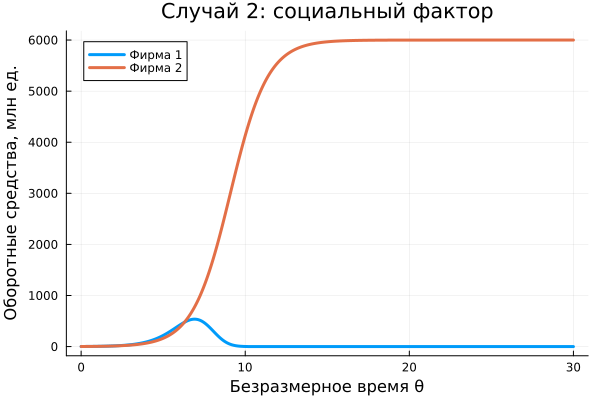
\includegraphics[width=1\linewidth,height=\textheight,keepaspectratio]{image/case2.png}
\end{column}
\end{columns}
\end{frame}

\begin{frame}{Что изменилось}
\protect\phantomsection\label{ux447ux442ux43e-ux438ux437ux43cux435ux43dux438ux43bux43eux441ux44c}
\textbf{Случай 1}

Обе фирмы растут и занимают свои части рынка.

\textbf{Случай 2}

Дополнительное влияние делает конкуренцию несимметричной.

Первая фирма после первоначального роста начинает терять оборотные
средства.

Вторая фирма сохраняет устойчивое положение.
\end{frame}

\begin{frame}{Сравнение}
\protect\phantomsection\label{ux441ux440ux430ux432ux43dux435ux43dux438ux435}
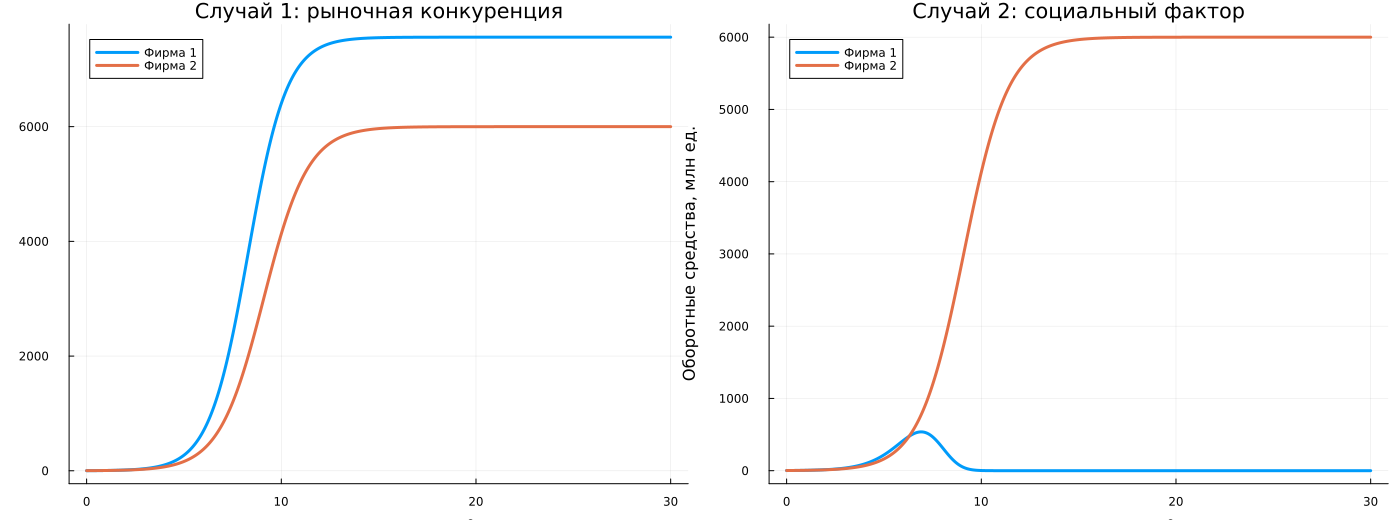
\includegraphics[width=0.78\linewidth,height=\textheight,keepaspectratio]{image/comparison.png}

Экономические исходные параметры одинаковы.

Главное отличие двух моделей --- дополнительный коэффициент
взаимодействия во втором случае.
\end{frame}

\begin{frame}{Итог}
\protect\phantomsection\label{ux438ux442ux43eux433}
Для варианта 2 реализованы две модели конкуренции фирм.

\begin{itemize}
\tightlist
\item
  при рыночной конкуренции обе фирмы сохраняются;
\item
  при дополнительном социально-психологическом воздействии первая фирма
  практически вытесняется с рынка.
\end{itemize}

\textbf{Характер взаимодействия конкурентов существенно влияет на
долгосрочную динамику оборотных средств.}
\end{frame}




\end{document}
